\section{Route Planning}
\label{sec:planning}

\subsection{Problem and design rationale}
Robot path planning can be done with many algorithms. Discrete methods such as Dijkstra~\cite{dijkstra1959note}, A*~\cite{hart1968astar} and Bellman-Ford search a graph; continuous sampling methods such as Rapidly-exploring Random Trees (RRT) and RRT* sample the free space. They trade off time complexity, space complexity, support for negative weights and optimality of the path.

In this project the arena is a known 2D map that fits a $40\times40$ grid, and the obstacles and observation stations are available to the program at run time. The station that shows the target, however, is unknown to the robot, so stations must be visited until the target is found. Navigation therefore reduces to repeated shortest-path queries on a known graph, followed by a visual check at each station.

\subsection{Map representation}
As mentioned, the obstacles and stations lie within a $40\times40$ grid at 0.1\,m per cell (385 occupied cells). The provided program includes a coordinate system and helpers that convert GPS positions to grid cells and back. The IMU yaw, rounded to the nearest multiple of $90^\circ$, gives the robot's grid heading. The planner rejects the two outermost rows and columns as a safety margin along the arena wall.

\subsection{Shortest path}
Given the problem and environment, we narrowed the choice to discrete methods, in particular Dijkstra and A*.

\lead{Why not sampling-based planners.} Sampling methods do not match the cell-based coordinate API we were given. They could arguably produce shorter paths, because they allow motion in any direction rather than the four directions and discrete cells we chose, but they are non-deterministic and need path smoothing. With the coordinate API and a generous 4-minute limit, we chose the simpler discrete approach. Incremental replanners such as D* Lite were also unnecessary: replanning happens only after a safety event, and a full replan takes well under a millisecond.

\lead{Why A*.} Among discrete methods we required a guaranteed shortest path. Depth-first search (DFS) gives no such guarantee and was excluded. Breadth-first search (BFS) does return shortest paths on our grid, where every move costs the same; in fact our Dijkstra on unit costs behaves like BFS with a priority queue. However, BFS stops being optimal as soon as moves have different costs, for example turn penalties or clearance costs, so we preferred a cost-based planner that extends to them. Bellman-Ford was ruled out because our costs are never negative, so its extra complexity buys nothing. Dijkstra and A* both return optimal paths when the A* heuristic never overestimates the true distance, which holds for the Manhattan distance on a 4-connected grid. We therefore chose between them by execution time (\cref{tab:planner-timing}).

\begin{table}[tbp]
  \centering\small
  \setlength{\tabcolsep}{4pt}
  \begin{tabular}{@{}lcccc@{}}
    \toprule
    Time (ms) & Mean & Median & Min & Max \\
    \midrule
    Dijkstra & 0.757 & 0.764 & 0.144 & 1.410 \\
    A*       & 0.208 & 0.153 & 0.026 & 0.767 \\
    \midrule
    Speed-up & \multicolumn{4}{c}{$3.65\times$ (by mean)} \\
    \bottomrule
  \end{tabular}
  \caption{Planner execution time over all 110 ordered start/station pairs on the $40\times40$ occupancy grid (25 repeats per pair, one CPU core). Both planners returned paths of identical, optimal length on every pair, and A* is 3.65$\times$ faster by mean time (median per-pair speed-up 4.2$\times$, range 1.7--10.3$\times$; \cref{app:planners}).}
  \label{tab:planner-timing}
\end{table}

As \cref{tab:planner-timing} shows, A* runs 3.65$\times$ faster than Dijkstra by mean time, and the per-pair median speed-up is 4.2$\times$. We therefore chose A*. Both planners finish in under a millisecond, while a mission takes 70--160\,s, so the speed-up has little effect on mission time. \Cref{app:planners} adds greedy best-first search, which is faster still but returns longer paths on 26 of 110 pairs, and a turn-penalised A* that keeps paths optimal while needing 47\% fewer turns.

\subsection{Station visiting order}
For the visiting order we chose a greedy nearest-neighbour rule. The planner keeps a list of all station coordinates and pops the nearest one (Manhattan distance from the robot's cell) as the next destination. TSP-style tours also exist, but the mission can end at any station before all have been visited, which makes nearest-neighbour search appealing. The resulting tours are fixed by the start position (\cref{fig:route}). Their cost shows in the student missions: from every start the target station S1 is reached only 7th or 8th, which sets their 130--162\,s mission times (\cref{fig:traj}).

We also considered an information-driven approach. An object detector would find station images anywhere in the robot's view, and stereo mapping would project each detection to world coordinates using the camera intrinsics and extrinsics, locating the station it belongs to. That station would then be removed from the list if it did not show the target, or visited directly if it did. However, the robot has no stereo or depth camera, so world coordinates cannot be recovered from a single detection.

\subsection{Motion execution}
Once a path is generated, the robot receives a list of discrete moves in the world frame. The problem then becomes turning a world direction such as ``UP'' into in-place rotations and forward moves. We solve it with rotation matrices: one for the desired global direction and one for the robot's current global direction. The goal is the rotation the robot must perform to face the desired direction.

This is similar to the extrinsic matrix in computer vision: we need the world direction as seen from the robot. The inverse of the robot's global direction serves as its extrinsic matrix. Multiplying it by the desired global direction gives that direction in the robot's frame, which is exactly the rotation the robot needs (straight, left, right or back).

Each forward move drives at full wheel speed until the GPS cell changes, while the safety layers (\cref{sec:safety}) monitor every simulation step. Each turn rotates in place until the IMU yaw is within 0.1\,rad of the next multiple of $90^\circ$. At the station, \texttt{go\_to\_yaw} turns the shorter way to the observation yaw, and the robot takes four frames at $\pm5^\circ$ and $\pm10^\circ$ for the classifier (\cref{sec:perception}). Raising the scan's wheel speed from 0.1 to 0.5\,rad/s, released together with the switch to A*, cut the worst-case mission time from 229\,s to 162\,s (\cref{tab:mc}).

\begin{figure*}[tbp]
  \centering
  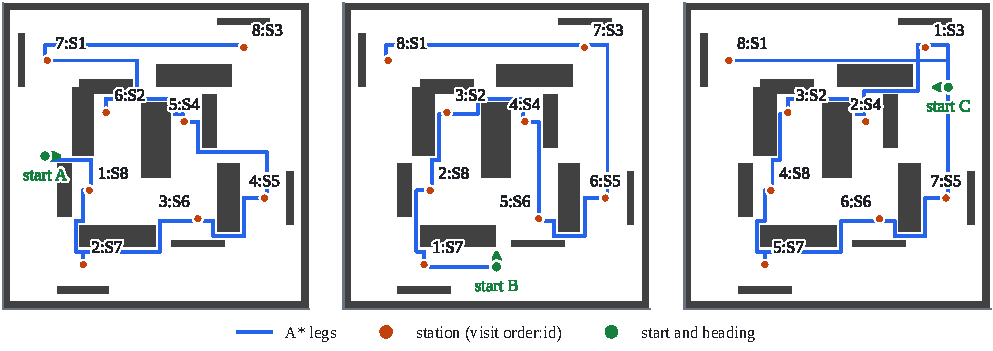
\includegraphics[width=\textwidth]{figs/route_planning.pdf}
  \caption{Greedy nearest-neighbour tours from (a) Start~A, (b) Start~B and (c) Start~C, produced by replaying the controller's station order and A* planner on the $40\times40$ occupancy grid (blue: A* legs between consecutive observation cells; labels: visit order and station; green arrow: start pose). The order is fixed by the start alone, and the mission stops at the first station showing the target, so mission time depends mainly on that station's position in the tour: S1, the student-mission target, comes 7th or 8th from every start.}
  \label{fig:route}
\end{figure*}
